\documentclass[a4paper,12pt,russian]{extarticle}
\usepackage{../MyPackages/commands}
\RequirePackage{caption}
\usepackage{graphicx}
\newcommand{\Pn}[3]{P^{(#1)} \br{#2,#3}}
\newcommand{\G}{\Gamma}
\newcommand{\e}{\eta_i^{(1)}}
\newcommand{\ee}{\eta_i^{(2)}}
\renewcommand{\b}{b^{(1)}}
\newcommand{\bb}{b^{(2)}}
\renewcommand{\P}[2]{P\br{\left. #1 \right| #2}}
\newcommand{\iakt}{[\tau_{i},\tau_{i+1})}
\newcommand{\Gr}[1]{\Gamma^{(#1)}}
\newcommand{\Mark}[0]{\brrr{\br{\G_i, \vk_{1,i}, \vk_{2,i}, \vk_{3,i}, \vk_{4,i}}, i \geqslant 0}}
%\newcommand{\Markk}[0]{\brrr{ \vk_i, i \geqslant 0}}
%\newcommand{\Markkhat}[0]{\brrr{ \hat{\vk}_i, i \geqslant 1}}
%\newcommand{\Markkhata}[0]{\brrr{ \hat{\vk}_i\br{a}, i \geqslant 1}}
%\newcommand{\Markkhato}[0]{\brrr{ \hat{\vk}_i\br{0}, i \geqslant 1}}
%\newcommand{\Markkhatoa}[0]{\brrr{ \hat{\hat{\vk}}_i\br{a}, i \geqslant 1}}
\usepackage[Magistr]{../MyPackages/ptvstyle}
%\selectlanguage{russian}
\title{Моделирование и анализ системы обслуживания конфликтных потоков в классе приоритетных алгоритмов}
\author{студент группы 85М1\\ Кочеганов В.~М.}
\advisor{к.ф.-м.н., доцент \\ Зорин А.~В.}
\chief{д.ф.-м.н., профессор \\ Федоткин М.~А.}
\date{2014}
\newcommand{\p}{\hat{p}}
\newcommand{\gam}[2]{\Gamma^{\left( #1 , #2 \right)} }
\newcommand{\T}[2]{T^{\left( #1 , #2 \right)} }
\newcommand{\ga}[1]{\Gamma^{\left( #1 \right)} }
\newcommand{\Tt}[1]{T^{\left( #1 \right)} }
\begin{document}

\section{Постановка задачи и построение математической модели}

\subsection{Постановка задачи на содержательном уровне}

Рассмотрим систему массового обслуживания следующего вида (Рис.~\ref{SystemScheme}).
\begin{figure}[h]
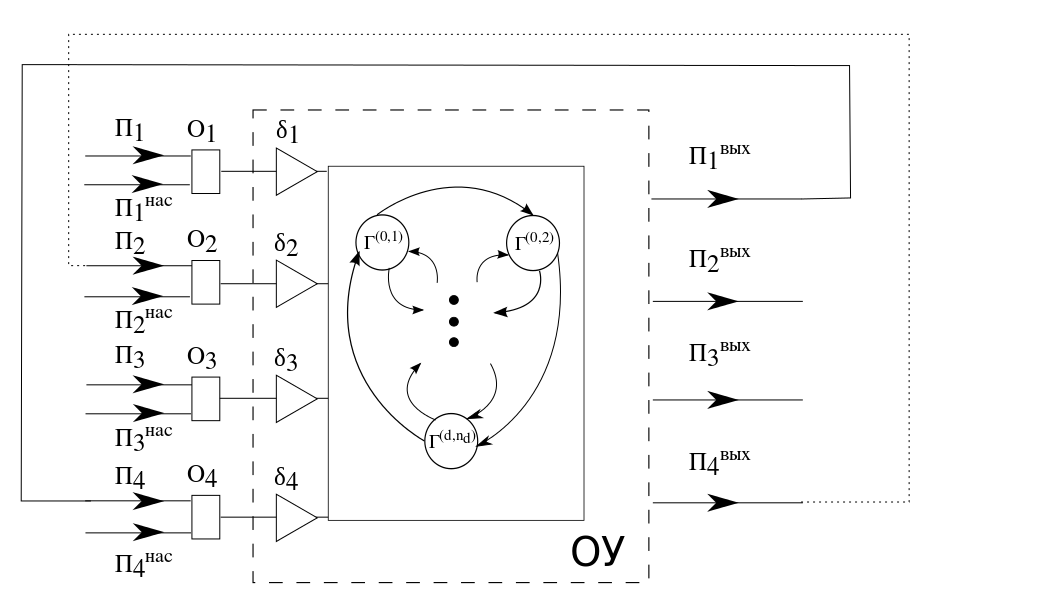
\includegraphics[scale=0.5]{SystemScheme.png} 
\caption{Структурная схема системы обслуживания}
\label{SystemScheme}
\end{figure}

Пусть в систему с одним обслуживающим устройством поступают потоки $\Pi_1$, $\Pi_2$, $\Pi_3$  и $\Pi_4$. Требования по потоку $\Pi_j$ становятся в соответствующую очередь $O_j$ с неограниченной вместимостью, $j\in \brrr{1, 2, 3, 4}$. Для $j \in \brrr{1, 2, 3}$ дисциплина очереди $O_j$, поддерживаемая устройством $\delta_j$, имеет тип FIFO (First In First Out). Таким образом, для обслуживания из соответствующей очереди выбирается то требование, которое пришло раньше. Дисциплина очереди $O_4$ будет описана ниже. Входные потоки $\Pi_1$ и $\Pi_3$ формируются внешней средой, которая, будем предполагать, имеет только одно состояние, то есть вероятностная структура потоков не меняется с течением времени. Требования потоков $\Pi_1$ и $\Pi_3$ формируют независимые между собой неординарные пуассоновские потоки, то есть  стационарные, без последействия и ординарные потоки групп требований. Интенсивности соответствующих простейших потоков для $\Pi_1$ и $\Pi_3$ будем обозначать $\la_1$ и $\la_3$, а распределение числа заявок в группе по потоку $\Pi_j$ будем описывать производящей функцией
\begin{equation}
f_j(z) = \sum_{\nu=1}^{\infty} p_{\nu}^{(j)} z ^{\nu}
\end{equation}
которая предполагается аналитической при $\forall z \colon |z|<(1+\varepsilon), \varepsilon > 0$ и $p_{\nu}^{(j)}>0$. Величина $p_{\nu}^{(j)}$ определяет вероятность того, что по потоку $\Pi_j$ число требований в группе равно $\nu$, $j\in \brrr{1,3}$. Обслуженные требования потока $\Pi_1$ поступают на повторное обслуживание, формируя при этом поток $\Pi_4$. Потоки $\Pi_2$ и $\Pi_3$ являются конфликтными, что означает запрет на одновременное обслуживание требований этих потоков и, следовательно, исследование системы не может быть сведено к задаче с меньшим числом потоков. 
 
 В каждый момент времени обслуживающее устройство находится в одном из конечного множества состояний $\Gamma=\{\G^{(k,r)} \colon k=0,1,\ldots,d; r=1,2,\ldots n_k\}$ с заданными натуральными числами $d$, $n_0$, $n_1$, $\ldots$, $n_d$. В каждом состоянии $\ga{k,r}$ обслуживающее устройство находится в течение времени $\Tt{k,r}$. Введем множества $\G^{\mathrm{I}}$, $\G^{\mathrm{II}}$, $\G^{\mathrm{III}}$ и $\G^{\mathrm{IV}}$ следующим образом. В состоянии $\gamma \in \G^{\mathrm{\Rmnum{1}}}$ обслуживаются только требования из очередей $O_1$, $O_2$ и $O_4$.
В состоянии $\gamma \in \G^{\mathrm{\Rmnum{2}}}$ обслуживаются только требования из очередей $O_2$ и $O_4$.
В состоянии $\gamma \in \G^{\mathrm{\Rmnum{3}}}$ обслуживаются только требования из очередей $O_1$, $O_3$ и $O_4$.
В состоянии $\gamma \in \G^{\mathrm{\Rmnum{4}}}$ обслуживаются только требования из очередей $O_3$ и $O_4$.
Тогда множество $\G$ есть объединение $\G = \G^{\mathrm{I}} \cup \G^{\mathrm{II}} \cup \G^{\mathrm{III}} \cup \G^{\mathrm{III}}$ непересекающихся подмножеств. 
Пусть ${}^1\G=\G^{\mathrm{\Rmnum{1}}} \cup \G^{\mathrm{\Rmnum{3}}}$, 
${}^2\G=\G^{\mathrm{\Rmnum{1}}} \cup \G^{\mathrm{\Rmnum{2}}}$,
${}^3\G=\G^{\mathrm{\Rmnum{3}}} \cup \G^{\mathrm{\Rmnum{4}}}$.

Смена состояний обслуживающего устройства осуществляется по следующему правилу. Множество состояний $C_k = \{\G^{(k,r)} \colon r=1,2,\ldots n_k\}$ будем называть $k$-м циклом, $k=1$, $2$, $\ldots$, $d$ (Рис. \ref{GraphScheme}). При $k=0$ состояние вида $\ga{0,r}$ будем называть состоянием продления, $r=0$, $1$, $\ldots$, $n_0$. Положим $r \oplus_k 1 = r+1$ для $r<n_k$ и $r \oplus_k 1 = 1$ при $r=n_k$, $k = 0$, $1$, $\ldots$, $d$. В цикле $C_k$ выделим подмножества $C_k^{\mathrm{O}}$ выходных, $C_k^{\mathrm{I}}$ входных и $C_k^{\mathrm{N}} = C_k \setminus (C_k^{\mathrm{O}} \cup C_k^{\mathrm{I}})$ нейтральных состояний. Тогда после состояния $\ga{k,r} \not\in C_k^{\mathrm{O}}$ обслуживающее устройство переходит в состояние $\ga{k,r \oplus_k 1}$ того же цикла $C_k$. При $\ga{k,r}$ принадлежащем множеству $C_k^{\mathrm{O}}$ прибор переходит в состояние $\ga{k,r\oplus_k 1}$, если число требований в очереди $O_3$ в момент переключения больше заданного порога $L$. В противном случае, то есть если число требований в очереди $O_3$ меньше либо равно $L$, то новое состояние прибора будет состоянием продления $\ga{0,r_1}$, где $r_1=h_1(\ga{k,r})$ и $h_1(\cdot)$~--- заданное отображение множества $\bigcup\limits_{k=1}^d C_k^{\mathrm{O}}$ во множество $\{1,2,\ldots, n_0\}$. После состояния $\ga{0,r}$ выбирается состояние того же вида $\ga{0,r_2}$, если число требований в очереди $O_3$ меньше $L$, где $r_2=h_2(r)$ и $h_2(\cdot)$~--- заданное отображение множества $\{1,2, \ldots, n_0\}$ на себя; в противном случае включается входное состояние $\ga{k,r_3} \in C_k^{\mathrm{I}}$, где $\ga{k,r_3}=h_3(r)$ и $h_3(\cdot)$~--- заданное отображение множества $\{1,2, \ldots, n_0\}$ на множество  $\bigcup\limits_{k=1}^d C_k^{\mathrm{I}}$. Считается, что все состояния продления $\ga{0,r} \in {}^2 \G$, все множества $C_k^\mathrm{O}\subset {}^2 \G$ и $C_k^\mathrm{I}\subset {}^3 \G$.

\begin{figure}[hb]\centering
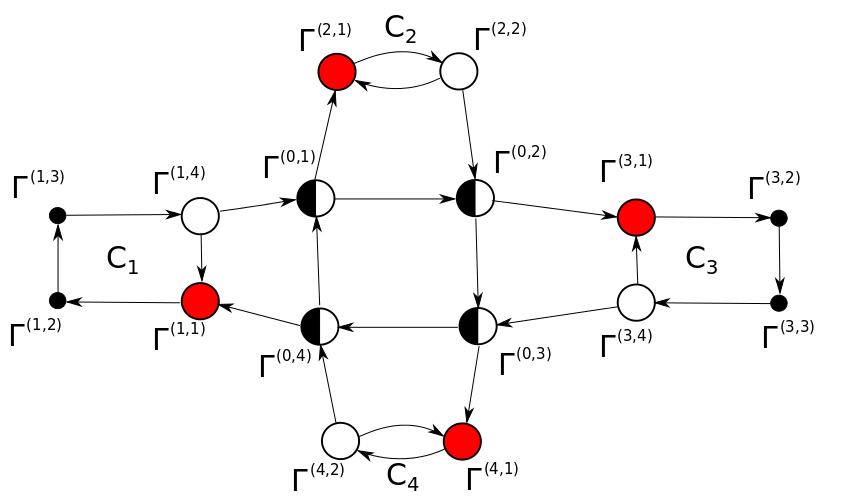
\includegraphics[scale=0.5]{GraphScheme3.png} 
\caption{Класс графов переходов. Незакрашенные вершины~--- выходные вершины, красным отмечены входные вершины, черным --- нейтральные, наполовину закрашенным вершинам соответствуют состояния продления}
\label{GraphScheme}
\end{figure}
%\subsection{Допустимые графы переходов состояний ОУ}

Рассмотрим введеные обозначения на примере Рис.~\ref{GraphScheme}. Примерами входных состояний являются $\ga{1,1} \in C_1^{\mathrm{I}}$ и $\ga{2,3} \in C_2^{\mathrm{I}}$, выходных состояний~--- $\ga{1,4} \in C_1^{\mathrm{O}}$ и $\ga{2,1} \in C_2^{\mathrm{O}}$, нейтральных состояний~--- $\ga{1,2}, \ga{1,3}, \ga{1,n_1} \in C_1^{\mathrm{N}}$ и $\ga{2,2} \in C_2^{\mathrm{N}}$. Состояния продления представлены на графе вершинами $\ga{0,1}$, $\ga{0,2}$, $\ga{0,3}$ и $\ga{0,4}$. Далее, отображение $h_1(\cdot)$ на графе задано таким образом, что оно переводит, например, выходное состояние $\ga{1,4}$ в число $1$~--- номер состояния продления $\ga{0,1}$, то есть $h_1(\ga{1,4})=1$. Аналогично $h_2(1)=2$, $h_2(2)=4$ и $h_2(3)=1$. Примером отображения $h_3(\cdot)$ является $h_3(2)=\ga{2,3}$.

Предполагается, что длительности обслуживания различных требований могут быть зависимыми и иметь различные законы распределения, поэтому вместо классического способа, состоящего в указании функции распределения длительности обслуживания произвольного требования, будут использованы потоки насыщения. Потоки насыщения $\Pi^{\mathrm{\text{нас}}}_j$, $j \in \brrr{1,2,3,4}$, определяются как виртуальные выходные потоки при 
условии максимального использования ресурсов обслуживающего устройства, а для $j\in \brrr{1, 2, 3}$ еще и при условии максимальной загрузки соответствующих очередей. 
Пусть поток насыщения $\Pi^{\mathrm{\text{нас}}}_j$, $j\in \brrr{1,2,3}$, будет содержать неслучайное число $\ell_{k,r,j}$ требований, обслуженных в течение времени $\Tt{k,r}$, если $\ga{k,r} \in~^j\G$, и будет содержать $0$ требований в противном случае: $\ga{k,r} \notin ~^j\G$. Пусть $Z_+$~--- множество целых неотрицательных чисел. Тогда, при условии, что в очереди $O_4$ находится $x \in Z_+$ требований, поток насыщения $\Pi^{\mathrm{\text{нас}}}_4$ определим как поток, содержащий все $x$ требований.
%\subsection{Пример: тандем из двух перекрестков} 
Наконец, при состоянии обслуживающего устройства $\ga{k,r}$ каждое требование из очереди $O_4$ с вероятностью $p_{k,r}$ и независимо от других завершает обслуживание и отправляется в очередь $O_2$ потока $\Pi_2$. С вероятностью $1-p_{k,r}$ требование очереди $O_4$ остается в ней до следующего такта.

В качестве наглядной физической интерпретации можно привести тандем из двух перекрестков (Рис. \ref{crossroads}).
\begin{figure}[h]
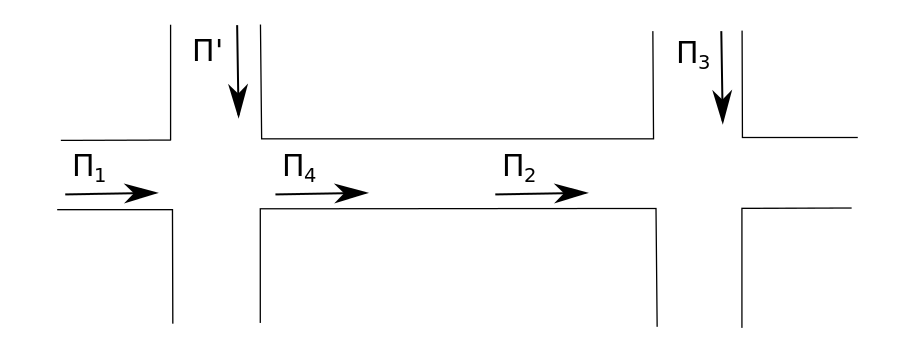
\includegraphics[scale=0.5]{Crossroads.png} 
\caption{Пример: тандем перекрестков}
\label{crossroads}
\end{figure}
В качестве потоков требований, формируемых внешней средой, выступают потоки прибывающих на перекрестки машин: конфликтные потоки $\Pi_1$, $\Pi_5$ на первом перекрестке, а также поток $\Pi_3$ на втором. Каждая машина из потока $\Pi_1$, проезжая первый перекресток, становится в очередь $O_4$ потока $\Pi_4$ и затем с некой вероятностью ($p_{k,r}$ для состояния $\ga{k,r}$ обслуживающего устройства) доезжает до следующего перекрестка, или же не успевает это сделать и остается в очереди $O_4$ до следующего такта обслуживания. В случае, если машина из очереди $O_4$ успевает доехать до второго перекрестка, она становится в очередь $O_2$ и ждет своей очереди для его прохождения.

Предполагается, что светофор на первом перекрестке имеет лишь два состояния: в первом состоянии машины потока $\Pi_1$ пропускаются фиксированное количество времени $\widetilde T^{\br{1,1}}$ (<<зеленый>> свет для $\Pi_1$); во втором --- простаивают в течение времени $\widetilde T^{\br{1,2}}$ (<<красный>> свет для $\Pi_1$). Светофор на втором перекрестке обслуживает по алгоритму с продлением: имеется два состояния обслуживания потока $\Pi_2$. Первое из них включается всегда после завершения обслуживания потока $\Pi_3$, а второе включается, если после очередного такта обслуживания потока $\Pi_2$ длина очереди $O_3$ не превосходит уровня $L$.
Длительности пребывания светофора на втором перекрестке в каждом из состояний суть $\widetilde T^{(2,1)}$, $\widetilde T^{(2,2)}$ и $\widetilde T^{(2,3)}$.

% В этом особом состоянии продления светофор продолжает пропускать машины потока $\Pi_3$ в течение фиксированного количества времени, вообще говоря, отличного от времени обслуживания в штатном режиме. В режим продления светофор переходит в случае, когда штатное обслуживание требований потока $\Pi_3$ закончено, однако количество требований (машин) в очереди $O_3$ еще превышает некий заданный порог $g$. В случае, если по истечении периода продления в очереди $O_3$ еще будет находиться достаточное число требований (превышающее заданный порог $L$), светофор проводит столько тактов продления дополнительно, сколько будет нужно для снижения количества машин в очереди $O_3$ до порога $L$.
%
Продемонстрируем на конкретном числовом примере выделение циклов и состояний продления.
 
Рассматривая тандем из двух перекрестков как единую систему массового обслуживания и предполагая наблюдение за ней только в (дискретные) моменты переключения состояния хотя бы одного из светофоров, может быть показано, что количество различных состояний у полученной системы конечно. Действительно, положим, например, за состояние объединенной системы вектор $\br{g^{(1)},g^{(2)}, f, t}$, где $g^{(j)}$~--- состояние $j$--го перекрестка, $f$~--- номер сменившего состояние перекрестка (принимает значение $0$ в случае, если сменили состояние оба перекрестка) и $t$~--- количество времени, оставшееся у продолжающего обслуживание с прошлого такта перекрестка. Тогда количество различных состояний не будет превышать величины  $2\times 3 \times 3 \times T$, где $T$~--- максимальная длительность нахождения каждого из светофоров в одном состоянии, поскольку первый перекресток может находиться только в одном из двух состояний, а второй~--- в одном из трех.

В завершение построения примера отметим, что при прохождении перекрестков машины предполагаются движущимися только в прямом направлении, то есть перемешивания конфликтных потоков не допускается. Таким образом, поток $\Pi'$ не представляет интереса для дальнейшего исследования системы и может быть отброшен и, следовательно, построенный пример целиком удовлетворяет структурной схеме на рис. \ref{SystemScheme}.
 
\subsection{Представление рассматриваемой системы обслуживания в виде кибернетической управляющей системы}
Описанная на содержательном уровне в предыдущем разделе система массового обслуживания должна рассматриваться как кибернетическая управляющая система обслуживания (ссылка на федоткина, Зорина А.В. киевский сборник твмс). Схема управляющей системы приведена на рис. \ref{SystemScheme}. На схеме присутствуют следующие блоки: 1) внешняя среда с одним состоянием; 2) входные полюса первого типа~--- входные потоки $\Pi_1$, $\Pi_2$, $\Pi_3$, $\Pi_4$; 3) входные полюса второго типа~--- потоки насыщения $\Pi_1^{\mathrm{\text{нас}}}$, $\Pi_2^{\mathrm{\text{нас}}}$, $\Pi_3^{\mathrm{\text{нас}}}$, $\Pi_4^{\mathrm{\text{нас}}}$; 4) внешняя память~--- очереди $O_1$, $O_2$, $O_3$, $O_4$; 5) устройство по переработки информации внешней памяти~--- устройства по поддержанию дисциплины очереди $\delta_1$, $\delta_2$, $\delta_3$, $\delta_4$; 6) внутренняя память обслуживающего устройства~--- обслуживающее устройство (ОУ); 7) устройство по переработке информации во внутренней памяти~--- граф смены состояний; 8) выходные полюса $\Pi_1^{\mathrm{\text{вых}}}$, $\Pi_2^{\mathrm{\text{вых}}}$, $\Pi_3^{\mathrm{\text{вых}}}$, $\Pi_4^{\mathrm{\text{вых}}}$. Координатой блока является номер этого блока на схеме. Для задания информации блоков введем следующие величины и укажем множество возможных состояний.

В качестве дискретной временной шкалы выберем последовательность $\tau_0=0$, $\tau_1$, $\tau_2$, $\ldots$ моментов смены состояний обслуживающего устройства. Обозначим $\G_i$ из множества $\G$ состояние обслуживающего устройства в течение времени $\left(\tau_{i-1};\tau_i\right]$, количество $\vk_{j,i} \in Z_+ $ требований в очереди $O_j$ в момент времени $\tau_i$, количество $\eta_{j,i} \in Z_+$ требований, поступивших в очередь $O_j$ по потоку $\Pi_j$ в течение времени $\left(\tau_{i};\tau_{i+1}\right]$, количество $\xi_{j,i} \in Z_+$ требований по потоку насыщения $\Pi^{\mathrm{\text{нас}}}_j$ в течение времени $\left(\tau_{i};\tau_{i+1}\right]$, количество $\overline{\xi}_{j,i}\in Z_+$ реально обслуженных требований по потоку $\Pi_j$ в течение времени $\left(\tau_{i};\tau_{i+1}\right]$.

Закон изменения состояния обслуживающего устройства будем предполагать заданным соотношением 
\begin{equation}
\G_{i+1}=h(\G_i,\vk_{3,i}).
\end{equation}
Для определения длительности $T_{i}$ состояния обслуживающего устройства в течение времени $\left(\tau_{i-1};\tau_i\right]$, удобно ввести функцию $h_T(\cdot,\cdot)$:
\begin{equation}
T_{i+1}=h_T(\G_i,\vk_{3,i})= \Tt{r'},\quad  \text{ где } \ga{r'}=h(\G_i,\vk_{3,i}).
\label{timeLaw}
\end{equation}
Функциональная зависимость
\begin{equation}
\overline{\xi}_{j,i}=\min\brrr{\vk_{j,i}+\eta_{j,i},\xi_{j,i}}
\label{saturationEq}
\end{equation}
между величиной $\overline{\xi}_{j,i}$ и величинами $\vk_{j,i}$, $\eta_{j,i}$, $\xi_{j,i}$ реализует стратегию механизма обслуживания требований, $j=1$,$2$,$3$. Далее, поскольку $\vk_{j,i+1}=\vk_{j,i}+\eta_{j,i}-\overline{\xi}_{j,i}$ для $j=1$,$2$,$3$,$4$, то из \eqref{saturationEq} следует соотношение
\begin{equation}
\vk_{j,i+1}=\max\brrr{{0,\vk_{j,i}+\eta_{j,i}-\xi_{j,i}}}.
\end{equation}
Из смысла поставленной задачи (см. также структурную схему \eqref{SystemScheme}) следуют соотношения для потока $\Pi_4$
\begin{equation}
\overline{\xi}_{4,i} = \eta_{2,i} \quad \eta_{4,i} = \overline{\xi}_{1,i}, \quad \vk_{4,i+1}=\vk_{4,i}+\eta_{4,i}-\overline{\xi}_{4,i}
\end{equation}

Нелокальное описание входных потоков и потоков насыщения состоит в указании некоторых свойств условных распределений выделенных дискретных компонент $\eta_i=(\eta_{1,i},\eta_{2,i}, \eta_{3,i}, \eta_{4,i})$ и $\xi_i=(\xi_{1,i}, \xi_{2,i}, \xi_{3,i}, \xi_{4,i})$ маркированных точечных процессов $\brrr{(\tau_i, \nu_i, \eta_i); i\geqslant 0}$ и $\brrr{(\tau_i, \nu_i, \xi_i); i\geqslant 0}$ при фиксированных значениях метки $\nu_i = \br{\Gamma_i,\vk_i}$, где $\vk_i=(\vk_{1,i}, \vk_{2,i}, \vk_{3,i}, \vk_{4,i})$.
%
%\item количество $\vk_{j,i} \in Z_+ $ требований в очереди $O_j$ в момент времени $\tau_i$;
%\item состояние обслуживающего устройства $\G_i\in \G = \brrr{\G^{(1)},\G^{(2)}, \ldots, \G^{(n)}}$ в течение времени $\left(\tau_{i-1};\tau_i\right]$;
%\item количество $\eta_{j,i}$ требований, поступивших в очередь $O_j$ по потоку $\Pi_j$ в течение времени $\left(\tau_{i};\tau_{i+1}\right]$;
%\item количество $\xi_{j,i}$ требований по потоку насыщения $\Pi^{\mathrm{sat}}_j$ в течение времени $\left(\tau_{i};\tau_{i+1}\right]$;
%\item количество $\overline{\xi}_{j,i}$ реально обслуженных требований по потоку $\Pi_j$ в течение времени $\left(\tau_{i};\tau_{i+1}\right]$.

Построим теперь 	вероятностное пространство $\br{\Omega, {\cal F}, P(\cdot)}$, для которого можно будет рассматривать введеные величины как случайные величины на этом пространстве. В соответствии с теоремой Ионеску Тулчи для этого достаточно задать вероятностное пространство $\br{\Omega_0, {\cal F}_0, P_0(\cdot)}$ и далее, считая для $0 \leqslant i < n$ и каждого набора элементарных исходов $(\omega_0, \omega_1, \ldots, \omega_{i-1})$ заданными пространства $\br{\Omega_i, {\cal F}_i, P_i(\omega_0,\omega_1,\ldots, \omega_{i-1},\cdot)}$, задать пространство $\br{\Omega_n, {\cal F}_n, P_n(\omega_0,\omega_1,\ldots, \omega_{n-1},\cdot)}$, причем для любого множества $B\in {\cal F}_i$ функции $P_i(\omega_0,\omega_1,\ldots, \omega_{i-1},B)$
должны быть измеримыми функциями от $(\omega_0, \omega_1, \ldots, \omega_{i-1})$. Тогда для $\Omega=\prod\limits_{i=0}^{\infty}\Omega_i$ и ${\cal F}=\prod\limits_{i=0}^{\infty} {\cal F}_i$ будет существовать единственная вероятностная мера $P(\cdot)$ такая, что $\forall i \geqslant 0$
\begin{equation}
P\brrr{\omega \colon \omega_0 \in A_0, \omega_1 \in A_1, \ldots, \omega_i\in A_i} = P_i\br{A_0 \times A_1 \times \ldots \times A_i},
\end{equation}
где 
\begin{equation}
 P_i\br{A_0 \times A_1 \times \ldots \times A_i} = \int_{A_0} P_0(d \omega_0) \int_{A_1} P(\omega_0,d \omega_1) \ldots \int_{A_i} P(\omega_0, \omega_1, \ldots, \omega_{i-1}, d \omega_i)
\end{equation}
и $A_k \in {\cal F}_k$, $k \geqslant 0$. Более того, наряду с вероятностной мерой $P(\cdot)$ на $(\Omega, {\cal F})$ также будет существовать случайная последовательность $X=\br{X_0(\omega), X_1(\omega), \ldots}$ такая, что
\begin{equation}
P\brrr{\omega \colon X_0(\omega) \in A_0, X_1(\omega)\in A_1, \ldots, X_i(\omega)\in A_i} = P_i\br{A_0\times A_1 \times \ldots, \times A_i},
\end{equation}
где $A_i\in {\cal F}_i$.

Итак, за описание элементарного исхода $\omega_i \in \Omega_i$ для произвольного $i \geqslant 0$ примем набор $\omega_i=(\eta_{1,i},\eta_{2,i}, \eta_{3,i})$. Таким образом, $\Omega_i=Z_+^3$, в качестве $\sigma$~--алгебр ${\cal F}_i$ возьмем множество всех подмножеств $\Omega_i$. Для задания вероятностных мер и случайных величин, упомянутых выше, введем следующие функции:
% и остается лишь задать вероятностные меры $P_0(\cdot)$ и $P_i(\omega_0,\omega_1,\ldots, \omega_{i-1},\cdot)$ для $i > 0$.
\begin{align}
f_{\xi_j | \G,\vk_3} (\gamma,x_3) &= \ell_{r,j},\text{ где }  h(\gamma,x)=\ga{r}\in {}^j\G \text{ и } j\in\brrr{1,2,3}\\
f_{\eta_4| \xi_1, \eta_1, \vk_1} (a,b,x) &= \begin{cases} a,\quad &\text{если }x+b\geq a \\  x+b,\quad &\text{если }x+b<a \end{cases},\\
P_{\eta_2|\G,\vk_3,\vk_4} (a,\gamma,x_3,x_4) &= \begin{cases} \binom{x_4}{a} p_r^a(1-p_r)^{x-a}, \quad &\text{если } h(\gamma,x_4)=\ga{r}, 0 \leqslant a \leqslant x_4 \\ 0, \quad &\text{иначе},\end{cases}, \\
P_{\eta_1|\G,\vk_3}(a,\gamma,x) &= \vp_1(a,h_T(\gamma,x)),\\
P_{\eta_3|\G,\vk_3}(a,\gamma,x) &= \vp_3(a,h_T(\gamma,x)),
\end{align}
где $a,b \in Z_+$, $\gamma \in \G$ и функции $\vp_1(\cdot,\cdot)$, $\vp_3(\cdot,\cdot)$ находятся из соотношений
\begin{equation}
\sum_{x=0}^{\infty} z^x\vp_j(x,t) = \exp\brrr{\la_j t \br{\sum_{b=1}^{\infty} z^b p_b^{(j)} -1}}, j \in \brrr{1,3}.
\end{equation}

Далее, зафиксируем $\gamma_0\in G$ и $(x_{1,0},x_{2,0},x_{3,0},x_{4,0})\in Z_+^4$, тогда  $P_0(\cdot)$ определим следующим образом:
\ml
{
P_0(a_1,a_2,a_3) = P_0\brrr{\omega_0=(\eta_{1,0},\eta_{2,0}, \eta_{3,0}) \colon \eta_{1,0}=a_1, \eta_{2,0}=a_2, \eta_{3,0}=a_3} = \\ 
=P_{\eta_1|\G,\vk_3}(a_1,\gamma_0,x_{3,0})\times P_{\eta_2|\G,\vk_3,\vk_4} (a_2,\gamma_0,x_{3,0},x_{4,0}) \times P_{\eta_3|\G,\vk_3}(a_3, \gamma_0, x_{3,0}).
}
На построенном вероятностном пространстве $\br{\Omega_0,{\cal F}_0,P_0(\cdot)}$ определим случайные величины
\begin{align}
\G_0&=\gamma_0=\mathrm{const},\\
\vk_{j,0}&=x_{j,0}=\mathrm{const},\\
\xi_{j,0}(\omega_0)&=f_{\xi_j | \G,\vk_3} (\gamma_0,x_{3,0})=\mathrm{const},\\
\eta_{j,0}(\omega_0)&=\eta_{j,0}(\eta_{1,0},\eta_{2,0},\eta_{3,0})=\eta_{j,0}, \\
\eta_{4,0}(\omega_0)&=f_{\eta_4| \xi_1, \eta_1, \vk_1} (\xi_{1,0}(\omega_0),\eta_{1,0}(\omega_0),x_{1,0}),\\
\overline{\xi}_{4,0}(\omega_0)&=\eta_{2,0}(\omega_0).
\end{align}
где $j\in \brrr{1,2,3}$.
Теперь, предполагая заданными вероятностные пространства $\br{\Omega_i, {\cal F}_i,P_i(\omega_0, \omega_1, \ldots, \omega_{i-1},\cdot)}$,$i\in \brrr{0,1,\ldots,n}$, случайные величины 
\begin{align}
\G_{i+1}(\omega_0,\omega_1,\ldots,\omega_{i+1})&=h\br{\G_{i}(\omega_0,\omega_1,\ldots,\omega_{i}),\vk_{3,i}(\omega_0,\omega_1,\ldots,\omega_{i})}=\mathrm{const},\\
\vk_{j,i+1}(\omega_0,\omega_1,\ldots,\omega_{i+1})&=\max\brrr{{0,\vk_{j,i}(\ldots)+\eta_{j,i}(\ldots)-\xi_{j,i}(\ldots)}}=\mathrm{const},\\
\vk_{4,i+1}(\omega_0,\omega_1,\ldots,\omega_{i+1})&=\vk_{4,i}(\ldots)+\eta_{4,i}(\ldots)-\overline{\xi}_{4,i}(\ldots),
\end{align}
на пространствах  $\br{\Omega_{i+1}, {\cal F}_{i+1},P_{i+1}(\omega_0, \omega_1, \ldots, \omega_{i},\cdot)}$, $i\in \brrr{0,1,\ldots,n-1}$, $j\in \brrr{1,2,3}$, и случайные величины 
\begin{align}
\xi_{j,i}(\omega_0,\omega_1,\ldots,\omega_i)&=f_{\xi_j | \G,\vk_3} (\G_i(\omega_0,\omega_1,\ldots,\omega_i),x_{3,i}(\omega_0,\omega_1,\ldots,\omega_i)),\\
\eta_{j,i}(\omega_0,\omega_1,\ldots,\omega_i)&=\eta_{j,i}(\omega_i)=\eta_{j,i}(\eta_{1,i},\eta_{2,i},\eta_{3,i})=\eta_{j,i}, \\
\eta_{4,i}(\omega_0,\omega_1,\ldots,\omega_i)&=f_{\eta_4| \xi_1, \eta_1, \vk_1} (\xi_{1,i}(\omega_0,\omega_1,\ldots,\omega_i),\eta_{1,i}(\omega_i),\vk_{1,i}(\omega_0,\omega_1,\ldots,\omega_i)),\\
\overline{\xi}_{4,0}(\omega_0,\omega_1,\ldots,\omega_i)&=\eta_{2,0}(\omega_i).
\end{align}
на пространствах  $\br{\Omega_{i}, {\cal F}_{i},P_{i}(\omega_0, \omega_1, \ldots, \omega_{i-1},\cdot)}$, $i\in \brrr{0,1,\ldots,n}$, $j\in \brrr{1,2,3}$, построим меру $P_{n+1}(\omega_0, \omega_1, \ldots, \omega_{n},\cdot)$:
\ml
{
P_{n+1}(\omega_0,\omega_1,\ldots,\omega_n,\brrr{\omega_{n+1} = (\eta_{1,n+1},\eta_{2,n+1},\eta_{3,n+1})\colon \eta_{1,n+1}=a_1, \eta_{2,n+1}=a_2, \eta_{3,n+1}=a_3}) = \\
=P_{\eta_1|\G,\vk_3}(a_1,\G_{n+1}(\omega_0,\omega_1,\ldots,\omega_i),\vk_{3,n+1}(\omega_0,\omega_1,\ldots,\omega_{i}))\times\\
\times P_{\eta_2|\G,\vk_3,\vk_4} (a_2,\G_{n+1}(\omega_0,\omega_1,\ldots,\omega_n),\vk_{4,n+1}(\omega_0,\omega_1,\ldots,\omega_{n})) \times\\
\times P_{\eta_3|\G,\vk_3}(a_3,\G_{n+1}(\omega_0,\omega_1,\ldots,\omega_i),\vk_{3,n+1}(\omega_0,\omega_1,\ldots,\omega_{i}))
}
%\ml
%{
%
%}
\subsection{Свойства условных распределений}

Все рассматриваемые в этой работе случайные элементы определяются на общем вероятностном пространстве $\br{\Omega, {\cal F}, P}$ элементарных исходов $\omega \in \Omega$ с вероятностной мерой $P(A)$, $A \in {\cal F}$, на $\sigma$-алгебре ${\cal F}$. 

Введем следующие случайные величины и элементы, $j \in \brrr{1,2,3,4}$:
\begin{itemize}
\item количество $\vk_{j,i} \in Z_+ $ требований в очереди $O_j$ в момент времени $\tau_i$;
\item состояние обслуживающего устройства $\G_i\in \G = \brrr{\G^{(1)},\G^{(2)}, \ldots, \G^{(n)}}$ в течение времени $\left(\tau_{i-1};\tau_i\right]$;
\item количество $\eta_{j,i}$ требований, поступивших в очередь $O_j$ по потоку $\Pi_j$ в течение времени $\left(\tau_{i};\tau_{i+1}\right]$;
\item количество $\xi_{j,i}$ требований по потоку насыщения $\Pi^{\mathrm{sat}}_j$ в течение времени $\left(\tau_{i};\tau_{i+1}\right]$;
\item количество $\overline{\xi}_{j,i}$ реально обслуженных требований по потоку $\Pi_j$ в течение времени $\left(\tau_{i};\tau_{i+1}\right]$.
\end{itemize}

Тогда для $j \in \brrr{1,2,3}$ имеем
\begin{equation}
\G_{i+1}=h(\G_i,\vk_{3,i}),\quad \vk_{j,i+1}=\max{\brrr{0,\vk_{j,i}+\eta_{j,i}-\xi_{j,i}}}, \quad \overline{\xi}_{j,i} = \min{\brrr{\xi_{j,i},\vk_{j,i}+\eta_{j,i}}}
\label{deterministicLawOne}
\end{equation}
и 
\begin{equation}
\eta_{2,i} = \overline{\xi}_{4,i}, \quad \eta_{4,i}=\overline{\xi}_{1,i}, \quad \vk_{4,i+1}=\vk_{4,i} + \overline{\xi}_{1,i} - \overline{\xi}_{4,i}
 \label{deterministicLawTwo}
\end{equation}
Также для определения длительности $T_{i}$ состояния обслуживающего устройства в течение $\left(\tau_{i-1};\tau_i\right]$, удобно ввести функцию $h_T(\cdot,\cdot)$:
\begin{equation}
T_{i+1}=h_T(\G_i,\vk_{3,i})= \Tt{r'},\quad  \text{ где } \ga{r'}=h(\G_i,\vk_{3,i}).
\label{timeLaw}
\end{equation}

Обозначим через $\vp_j(x,t)$, $j\in \brrr{1,3}$, условную вероятность того, что за время $t>0$ по потоку $\Pi_j$ поступит ровно $b\in Z_+$ требований:
\begin{equation}
\P{ \eta_{j,i} = b}{\G_i=\ga{k,r}, \vk_{3,i}=x}=\vp_j(b,h_T (\ga{k,r}, x)).
\end{equation}
Учитывая закон распределения процесса Пуассона и количества требований в пачках, величины $\vp_j(x,t)$ могут быть найдены из соотношений
\begin{equation}
\sum_{x=0}^{\infty} z^x\vp_j(x,t) = \exp\brrr{\la_j t \br{\sum_{b=1}^{\infty} z^b \pi(b,j) -1}}.
\end{equation}

Для потоков насыщения имеем следующие соотношения:
\begin{align}
\P{\xi_{j,i} = 0}{\G_i=\ga{k,r}, \vk_{3,i} = x} = 1, &\quad \G_{i+1} \notin~^j\G,\\
\P{\xi_{j,i} = \ell_{r',j}}{\G_i=\ga{k,r}, \vk_{3,i} = x} = 1, &\quad \G_{i+1}=\ga{r'}\in~^j\G,
\end{align}
где $j\in \{1, 2, 3\}$, $x \in Z_+$.


Введем для $0 < u \leqslant 1$ и $0 \leqslant k \leqslant x$ величину
\begin{equation}
\psi\br{k,x,u} = C_x^k u^k (1-u)^{x-k}.
\end{equation}
Поскольку требования из очереди $O_4$ независимо друг от друга с вероятностью $p_{k,r}$ на выходе системы поступают в очередь $O_2$, то количество требований в выходном потоке $\Pi_4^{\mathrm{\text{вых}}}$ определяется по биномиальному закону распределения:
\begin{equation}
\P{\overline{\xi}_{4,i} = b}{ \G_i = \ga{k,r}, \vk_{4,i}=x, \vk_{3,i}=\tilde{x}}=\psi\br{b,x,p_{r'}}, \quad \G_{i+1}=\ga{r'}, \quad 0 \leqslant b \leqslant x.
\end{equation}


Введем следующие события:
\begin{align}
A_i\br{r;x_1;x_2;x_3;x_4} &= \brrr{\G_i=\ga{k,r},\vk_{3,i}=x_3}\bigcap \brrr{\vk_{1,i}=x_1,\vk_{2,i}=x_2,\vk_{4,i}=x_4}\\
B_i\br{b_1;b_3;y_1;y_2;y_3;y_4} &= \brrr{\eta_{1,i}=b_1,\eta_{3,i}=b_3} \bigcap \brrr{\xi_{1,i}=y_1,\xi_{2,i}=y_2,\xi_{3,i}=y_3,\overline{\xi}_{4,i}=y_4}
\end{align}

В соответствии с описанной структурой системы, количество требований пришедших по потокам $\Pi_1$, $\Pi_3$, $\Pi_1^{\mathrm{\text{нас}}}$,  $\Pi_2^{\mathrm{\text{нас}}}$, $\Pi_3^{\mathrm{\text{нас}}}$ и $\Pi_4^{\mathrm{\text{вых}}}$ за $(i+1)$-ый такт зависит только от состояния обслуживающего устройства и размера очередей в момент $\tau_i$. Поэтому условные распределения рассматриваемых в системе потоков, учитывая все <<прошлое>> системы удовлетворяют соотношениям
\ml
{
\P{B_i\br{b_1;b_3;y_1;y_2;y_3;y_4}}{\bigcap_{t=0}^{i} A_t\br{r_t;x_{1,t};x_{2,t};x_{3,t};x_{4,t}}} = \\
\P{B_i\br{b_1;b_3;y_1;y_2;y_3;y_4}}{A_i\br{r_i;x_{1,i};x_{2,i};x_{3,i};x_{4,i}}}
%= \P{\eta_{1,i}=b_1, \eta_{3,i}=b_3, \xi_{1,i}=y_1, \xi_{2,i}=y_2, \xi_{3,i}=y_3;\overline{\xi}_{4,i}=y_4}{\G_i=\ga{r_i},\vk_{3,i}=x_{3,i}}=\\
%= \P{\eta_{1,i}=b_1}{\G_i=\ga{r_i},\vk_{3,i}=x_{3,i}} \times
%\P{\eta_{2,i}=b_2}{\G_i=\ga{r_i},\vk_{3,i}=x_{3,i}} \times \\
%\P{\eta_{3,i}=b_3}{\G_i=\ga{r_i},\vk_{3,i}=x_{3,i}} \times 
%\P{\xi_{1,i}=y_1}{\G_i=\ga{r_i},\vk_{3,i}=x_{3,i}} \times \\
%\P{\xi_{2,i}=y_2}{\G_i=\ga{r_i},\vk_{3,i}=x_{3,i}} \times 
%\P{\xi_{3,i}=y_3;\overline{\xi}_{4,i}=y_4}{\G_i=\ga{r_i},\vk_{3,i}=x_{3,i}}
}
Далее, в силу того, что потоки насыщения $\Pi_1^{\mathrm{\text{нас}}}$,  $\Pi_2^{\mathrm{\text{нас}}}$, $\Pi_3^{\mathrm{\text{нас}}}$, входные потоки $\Pi_1$, $\Pi_3$, а также выходной поток $\Pi_4^{\mathrm{\text{вых}}}$ условно независимы между собой, верно следующее соотношение:
\ml
{
\label{etaXiIndependence}
\P{B_i\br{b_1;b_3;y_1;y_2;y_3;y_4}}{\bigcap_{t=0}^{i} A_t\br{r_t;x_{1,t};x_{2,t};x_{3,t};x_{4,t}}} = \\
= \P{\eta_{1,i}=b_1}{\G_i=\ga{r_i},\vk_{3,i}=x_{3,i}} \times 
\P{\eta_{3,i}=b_3}{\G_i=\ga{r_i},\vk_{3,i}=x_{3,i}} \times \\
\P{\xi_{1,i}=y_1}{\G_i=\ga{r_i},\vk_{3,i}=x_{3,i}} \times 
\P{\xi_{2,i}=y_2}{\G_i=\ga{r_i},\vk_{3,i}=x_{3,i}} \times \\
\P{\xi_{3,i}=y_3;\overline{\xi}_{4,i}=y_4}{\G_i=\ga{r_i},\vk_{3,i}=x_{3,i}} \times
\P{\overline{\xi}_{4,i}=y_4}{\G_i=\ga{r_i},\vk_{3,i}=x_{3,i},\vk_{4,i} = x_{4,i}}
}

Сформулируем и докажем теорему о марковости последовательности $\Mark$:
\begin{theorem}
При заданном распределении начального вектора $\br{\G_0,\vk_{1,0},\vk_{2,0},\vk_{3,0},\vk_{4,0}}$ последовательность $\Mark$ является цепью Маркова. 
\end{theorem}

\begin{proof}
Для доказательства достаточно показать, что 
\ml
{
\P{A_{i+1}\br{r;x_{1};x_{2};x_{3};x_{4}}}{\bigcap_{t=0}^{i} A_t\br{r_t;x_{1,t};x_{2,t};x_{3,t};x_{4,t}}} = \\
\P{A_{i+1}\br{r;x_{1};x_{2};x_{3};x_{4}}}{ A_i\br{r_i;x_{1,i};x_{2,i};x_{3,i};x_{4,i}}}
\label{markovToProve}
}
Распишем сначала левую часть равенства \eqref{markovToProve}. Учитывая то, что сумма непересекающихся событий $B_i\br{b_1;b_3;y_1;y_2;y_3;y_4}$ есть достоверное событие, $\cup_{b,y} B_i\br{b_1;b_3;y_1;y_2;y_3;y_4}=\Omega$ получим

\ml
{
\P{A_{i+1}\br{r;x_{1};x_{2};x_{3};x_{4}}}{\bigcap_{t=0}^{i} A_t\br{r_t;x_{1,t};x_{2,t};x_{3,t};x_{4,t}}} = \\
=\sum_{b,y}\P{A_{i+1}\br{r;x_{1};x_{2};x_{3};x_{4}} \bigcap B_i\br{b_1;b_3;y_1;y_2;y_3;y_4}}{\bigcap_{t=0}^{i} A_t\br{r_t;x_{1,t};x_{2,t};x_{3,t};x_{4,t}}} = \\
= \sum_{b,y}\P{B_i\br{b_1;b_3;y_1;y_2;y_3;y_4}}{\bigcap_{t=0}^{i} A_t\br{r_t;x_{1,t};x_{2,t};x_{3,t};x_{4,t}}}\times\\
\times \P{A_{i+1}\br{r;x_{1};x_{2};x_{3};x_{4}}}{\bigcap_{t=0}^{i} A_t\br{r_t;x_{1,t};x_{2,t};x_{3,t};x_{4,t}}\bigcap B_i\br{b_1;b_3;y_1;y_2;y_3;y_4}}
\label{markovProof}
}
Беря во внимание \eqref{deterministicLawOne} и \eqref{deterministicLawTwo}, найдем второй множитель:
\ml
{
\P{A_{i+1}\br{r;x_{1};x_{2};x_{3};x_{4}}}{\bigcap_{t=0}^{i} A_t\br{r_t;x_{1,t};x_{2,t};x_{3,t};x_{4,t}}\bigcap B_i\br{b_1;b_3;y_1;y_2;y_3;y_4}} = \\
= P\left(\G_{i+1}=\ga{k,r},\vk_{1,i+1}=x_1,\vk_{2,i+1}=x_2,\vk_{3,i+1}=x_3,\vk_{4,i+1}=x_4\right| \bigcap_{t=0}^{i-1} A_t\br{r_t;x_{1,t};x_{2,t};x_{3,t};x_{4,t}} \bigcap \\ \bigcap 
\brrr{\G_i=\ga{r_i},\vk_{1,i}=x_{1,i},\vk_{2,i}=x_{2,i},\vk_{3,i}=x_{3,i},\vk_{4,i}=x_{4,i}} \bigcap \\
\bigcap \left. \brrr{\eta_{1,i}=b_1,\eta_{3,i}=b_3,\xi_{1,i}=y_1,\xi_{2,i}=y_2,\xi_{3,i}=y_3;\overline{\xi}_{4,i}=y_4}
\right) = \\
= P\left(h\br{\ga{r_i},x_{3,i}}=\ga{k,r},
\max{\brrr{0,x_{1,i}+b_1-y_1}}=x_1,\right.\\
\max{\brrr{0,x_{2,i}+y_4-y_2}}=x_2, 
\max{\brrr{0,x_{3,i}+b_3-y_3}}=x_3,
x_{4,i}+\min{\brrr{y_1,x_{1,i}+b_1}} - \overline{\xi}_{4,i}=x_4\left.
\right| \\
\bigcap_{t=0}^{i-1} A_t\br{r_t;x_{1,t};x_{2,t};x_{3,t};x_{4,t}} \bigcap
\brrr{\G_i=\ga{r_i},\vk_{1,i}=x_{1,i},\vk_{2,i}=x_{2,i},\vk_{3,i}=x_{3,i},\vk_{4,i}=x_{4,i}} \bigcap \\
\bigcap \left. \brrr{\eta_{1,i}=b_1,\eta_{3,i}=b_3,\xi_{1,i}=y_1,\xi_{2,i}=y_2,\xi_{3,i}=y_3;\overline{\xi}_{4,i}=y_4}
\right) = \\ 
= P\left(h\br{\ga{r_i},x_{3,i}}=\ga{k,r},
\max{\brrr{0,x_{1,i}+b_1-y_1}}=x_1,\right.\\
\max{\brrr{0,x_{2,i}+y_4-y_2}}=x_2, 
\max{\brrr{0,x_{3,i}+b_3-y_3}}=x_3,
x_{4,i}+\min{\brrr{y_1,x_{1,i}+b_1}} - \overline{\xi}_{4,i}=x_4\left.\right),
\label{markovProoff}
}
где последнее равенство верно, поскольку оставшаяся под знаком вероятности величина уже не является случайной. Из \eqref{etaXiIndependence}, \eqref{markovProof} и  \eqref{markovProoff} получаем выражение для левой части равенства \eqref{markovToProve}:

\ml
{
\P{A_{i+1}\br{r;x_{1};x_{2};x_{3};x_{4}}}{\bigcap_{t=0}^{i} A_t\br{r_t;x_{1,t};x_{2,t};x_{3,t};x_{4,t}}} = \\
=  \sum_{b,y}\P{\eta_{1,i}=b_1,  \eta_{3,i}=b_3, \xi_{1,i}=y_1, \xi_{2,i}=y_2, \xi_{3,i}=y_3;\overline{\xi}_{4,i}=y_4}{\G_i=\ga{r_i},\vk_{3,i}=x_{3,i}}\times\\
\times  P\left(h\br{\ga{r_i},x_{3,i}}=\ga{k,r},
\max{\brrr{0,x_{1,i}+b_1-y_1}}=x_1,\right.\\
\max{\brrr{0,x_{2,i}+y_4-y_2}}=x_2, 
\max{\brrr{0,x_{3,i}+b_3-y_3}}=x_3,
x_{4,i}+\min{\brrr{y_1,x_{1,i}+b_1}} - \overline{\xi}_{4,i}=x_4\left.\right)
}

Заметим, что в наших рассуждениях мы нигде не использовали информацию о событиях \par $\bigcap_{t=0}^{i-1} A_t\br{r_t;x_{1,t};x_{2,t};x_{3,t};x_{4,t}}$, поэтому рассуждения для правой части \eqref{markovToProve} будут аналогичными:

\mll
{
\P{A_{i+1}\br{r;x_{1};x_{2};x_{3};x_{4}}}{ A_i\br{r_i;x_{1,i};x_{2,i};x_{3,i};x_{4,i}}} = \\
= \sum_{b,y}\P{B_i\br{b_1;b_3;y_1;y_2;y_3;y_4}}{ A_i\br{r_i;x_{1,i};x_{2,i};x_{3,i};x_{4,i}}}\times\\
\times \P{A_{i+1}\br{r;x_{1};x_{2};x_{3};x_{4}}}{ A_i\br{r_i;x_{1,i};x_{2,i};x_{3,i};x_{4,i}}\bigcap B_i\br{b_1;b_3;y_1;y_2;y_3;y_4}} = \\
= \sum_{b,y}\P{\eta_{1,i}=b_1,  \eta_{3,i}=b_3, \xi_{1,i}=y_1, \xi_{2,i}=y_2, \xi_{3,i}=y_3;\overline{\xi}_{4,i}=y_4}{\G_i=\ga{r_i},\vk_{3,i}=x_{3,i}}\times \\
\times 
P\left(\G_{i+1}=\ga{k,r},\vk_{1,i+1}=x_1,\vk_{2,i+1}=x_2,\vk_{3,i+1}=x_3,\vk_{4,i+1}=x_4\right|  \\ 
\brrr{\G_i=\ga{r_i},\vk_{1,i}=x_{1,i},\vk_{2,i}=x_{2,i},\vk_{3,i}=x_{3,i},\vk_{4,i}=x_{4,i}} \bigcap \\
\bigcap \left. \brrr{\eta_{1,i}=b_1,\eta_{3,i}=b_3,\xi_{1,i}=y_1,\xi_{2,i}=y_2,\xi_{2,i}=y_2,\xi_{3,i}=y_3;\overline{\xi}_{4,i}=y_4}
\right) = 
}

откуда опять в силу \eqref{deterministicLawOne} и \eqref{deterministicLawTwo} получаем
\mll
{
=\sum_{b,y}\P{\eta_{1,i}=b_1,  \eta_{3,i}=b_3, \xi_{1,i}=y_1, \xi_{2,i}=y_2, \xi_{3,i}=y_3;\overline{\xi}_{4,i}=y_4}{\G_i=\ga{r_i},\vk_{3,i}=x_{3,i}}\times \\
\times P\left(h\br{\ga{r_i},x_{3,i}}=\ga{k,r},
\max{\brrr{0,x_{1,i}+b_1-y_1}}=x_1,\right.\\
\max{\brrr{0,x_{2,i}+y_4-y_2}}=x_2, 
\max{\brrr{0,x_{3,i}+b_3-y_3}}=x_3,
x_{4,i}+\min{\brrr{y_1,x_{1,i}+b_1}} - \overline{\xi}_{4,i}=x_4\left.\right).
}
Таким образом, выражения для левой и правой частей \eqref{markovToProve} совпадают, следовательно равенство верно и последовательность $\Mark$ является цепью Маркова.
\end{proof}


\end{document}






\subsection{Постановка задачи}

\begin{figure}[h]
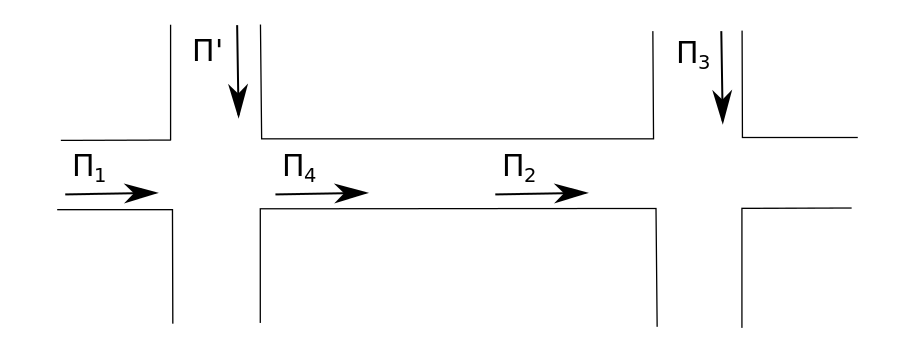
\includegraphics[scale=0.5]{Crossroads.png} 
\end{figure}

\begin{figure}[h]
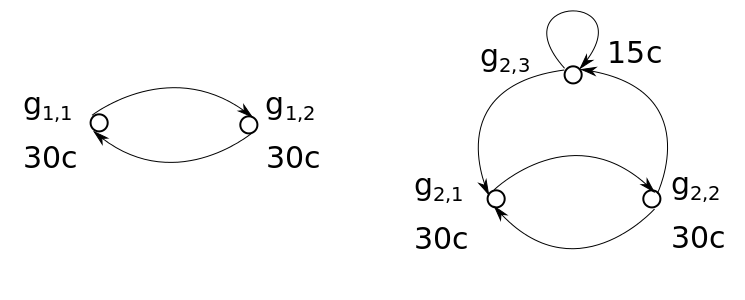
\includegraphics[scale=0.5]{SystemStates.png} 
\end{figure}



Требования по потокам $\Pi_j$, $j=1,2,4$, поступают пачками, причем пачки поступают в соответствии с Пуассоновским процессом с параметром $\la_j$. Требования из потока $\Pi_1$, будучи обслуженными, образуют поток $\Pi_3$.
Требования по потоку $\Pi_j$ поступают в соответствующую очередь $O_j$, $j=\overline{1,4}$.

Первый перекресток может находиться в одном из двух состояний:
\begin{itemize}
\item обслуживать поток $\Pi_1$ (состояние $\gam{1}{1}$ длительностью $\T{1}{1}$) и 
\item
обслуживать поток $\Pi_2$ (состояние $\gam{1}{2}$ длительностью $\T{1}{2}$).
\end{itemize}

Второй перекресток имеет три состояния:
\begin{itemize}
\item обслуживание потока $\Pi_3$ (состояние $\gam{2}{1}$ длительностью $\T{2}{1}$);
\item обслуживание потока $\Pi_4$ (состояние $\gam{2}{2}$ длительностью $\T{2}{2}$) и
\item продолжение обслуживания потока $\Pi_4$ в случае 
превышения объема оставшейся очереди $O_4$ некого порога (состояние $\gam{2}{3}$ длительностью $\T{2}{3}$);
\end{itemize}

Объединим рассматриваемые обслуживающие устройства в одно, состояние которого опишем с помощью вектора из множества $S_{general}\left(\Gamma^{(1,i_1)}; \Gamma^{(2,i_2)}; T\right)$, где $i_1\in \left\{1,2\right\}$, $i_2 \in \left\{1,2,3\right\}$, $T\in \left\{1, 2, \ldots, \max_{i_1,i_2}{\left(T^{(1,i_1)}, T^{(2,i2)}\right)}\right\}$. Свое состояние новое устройство меняет в моменты смены состояний одного из составляющих его устройств.

\begin{theorem}
Количество состояний полученного обслуживающего устройства конечно
\end{theorem}
\begin{proof}
Поскольку множество различных состояний $\Gamma$, в которые обслуживающее устройство может совершить переход, является подмножеством $S_{general}$ ($S \subset S_{general}$), то
\begin{equation*}
\left|S\right| \leqslant \left|S_{general}\right| = 2\times 3 \times \max_{i_1,i_2}{\left(T^{(1,i_1)}, T^{(2,i2)}\right)}
\end{equation*}
\end{proof}

В следствие этого результата мы можем перенумеровать состояния $\G = \brrr{\G^{(1)},\G^{(2)}, \ldots, \G^{(n)}}$, а также соответствующие им длительности $T=\brrr{T^{(1)},T^{(2)}, \ldots, T^{(n)}}$.
Каждое состояние $\G^{(r)}$ принадлежит одному из следующих четырех классов $\G^{\mathrm{\Rmnum{1}}}$, $\G^{\mathrm{\Rmnum{2}}}$, $\G^{\mathrm{\Rmnum{3}}}$ и $\G^{\mathrm{\Rmnum{4}}}$.
\begin{itemize}
\item в состоянии $\G^{(r)} \in \G^{\Rmnum{1}}$ обслуживаются только требования из очередей $O_1$ и $O_3$;
\item в состоянии $\G^{(r)} \in \G^{\Rmnum{2}}$ обслуживаются только требования из очередей $O_1$ и $O_4$;
\item в состоянии $\G^{(r)} \in \G^{\Rmnum{3}}$ обслуживаются только требования из очередей $O_2$ и $O_3$;
\item в состоянии $\G^{(r)} \in \G^{\Rmnum{4}}$ обслуживаются только требования из очередей $O_2$ и $O_4$.
\end{itemize}

Для описания процесса обслуживания будут также использоваться потоки насыщения $\Pi^{\mathrm{sat}}_j$, $j=\overline{1,4}$, определяемые как выходные потоки при максимальной загруженности обслуживающего устройства. Пусть
\begin{itemize}
\item для $j=1$ $^j\G=\G^{\Rmnum{1}} \cup \G^{\Rmnum{2}}$;
\item для $j=2$ $^j\G=\G^{\Rmnum{3}} \cup \G^{\Rmnum{4}}$;
\item для $j=3$ $^j\G=\G^{\Rmnum{1}} \cup \G^{\Rmnum{3}}$;
\item для $j=4$ $^j\G=\G^{\Rmnum{2}} \cup \G^{\Rmnum{4}}$;
\end{itemize}
Тогда поток насыщения $\Pi^{\mathrm{sat}}_j$ будет содержать неслучайное число $l_{r,j}$ требований, обслуженных в течение времени $\Tt{k,r}$, если $\ga{k,r} \in ^j\G$, и не будет содержать требований в противном случае, $\ga{k,r} \notin ^j\G$. 

Моменты $\tau_0 = 0, \tau_1, \ldots$ наблюдения за системой положим совпадающими с моментами переключения состояния обслуживающего устройства. Определим следующие случайные величины и элементы:
\begin{itemize}
\item количество $\vk_{j,i} \in Z_+ $ требований в очереди $O_j$ в момент времени $\tau_i$;
\item состояние обслуживающего устройства $\G_i\in \G = \brrr{\G^{(1)},\G^{(2)}, \ldots, \G^{(n)}}$ в течение $\left(\tau_{i-1};\tau_i\right]$;
\item количество $\eta_{j,i}$ требований, поступивших в очередь $O_j$ по потоку $\Pi_j$ в течение $\left(\tau_{i};\tau_{i+1}\right]$;
\item количество $\xi_{j,i}$ требований по потоку насыщения $\Pi^{\mathrm{sat}}_j$ в течение $\left(\tau_{i};\tau_{i+1}\right]$;
\item количество $\overline{\xi_{j,i}}$ реально обслуженных требований по потоку $\Pi_j$,
\end{itemize}
для $j=\overline{1,4}$.






В данной работе будет применен так называемый кибернетический подход, который предполагает, что наблюдение за системой осуществляется в дискретные моменты времени $\tau_0 = 0,~ \tau_1,~ \ldots$,~  совпадающие с моментами переключения состояния обслуживающего устройства. 
Будем считать, что функция перехода из состояния $\G_i$ в момент $\tau_i$ в состояние $\G_{i+1}$ в момент $\tau_{i+1}$ известна и задается функцией $h(\G_i,x_i)$ от предыдущего состояния $\G_i$ и величины $x_i$ очереди $O_3$ в момент $\tau_i$. Таким образом, обслуживающее устройство, в зависимости от объема очереди $O_3$, может переходить в разные состояния, что влечет за собой особый класс рассматриваемых графов переходов. Опишем сейчас общую структуру класса ${\cal K}$ рассматриваемых графов переходов между состояниями обслуживающего устройства (ОУ).

Первое и самое очевидное требование, которое мы наложим на рассматриваемый класс графов, --- это ориентированность и связность. Порядок прохождения состояний ОУ имеет значение и рассматривать недостижимые состояния (которые делают граф несвязным) не имеет смысла.

Далее, будем предполагать, что каждый граф $G$ из класса ${\cal K}$ может быть построен по следующему алгоритму.
\begin{enumerate}
\item Выделить из множества всех вершин графа $d$ непересекающихся кластеров вершин $C_1$, $C_2$, $\ldots$, $C_d$ таким образом, чтобы вершины внутри кластеров были соединены в цикл. Каждый кластер $C_j$ в свою очередь разделить на три непересекающихся множества вершин $C_j=C_j^{\mathrm{I}} + C_j^{\mathrm{O}} + C_j^{\mathrm{N}}$. Множество $C_j^{\mathrm{I}}$ будем называть множеством входных вершин, $C_j^{\mathrm{O}}$~--- множеством выходных вершин и $C_j^{\mathrm{N}}$~--- множеством нейтральных вершин. (Рис.~\ref{GraphSchemeOne}).

\begin{figure}[h]
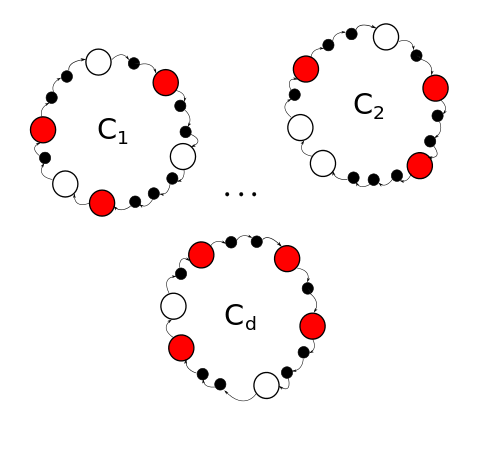
\includegraphics[scale=0.4]{GraphScheme1.png} 
\caption{Класс графов переходов (Шаг 1). Незакрашенные вершины --- выходные вершины, красным отмечены входные вершины, черным --- нейтральные}
\label{GraphSchemeOne}
\end{figure}
\item Каждое выходное состояние $c_1$ некоего кластера $C_j$ может быть соединено с входным состоянием того же или другого кластера $C_k$ постредством сторонней вершины $c$, не принадлежащей никакому из кластеров $C_1$, $C_2$, $\ldots$, $C_d$, и двух соединящих ребер (Рис.~\ref{GraphSchemeTwo}).
\begin{figure}[h]
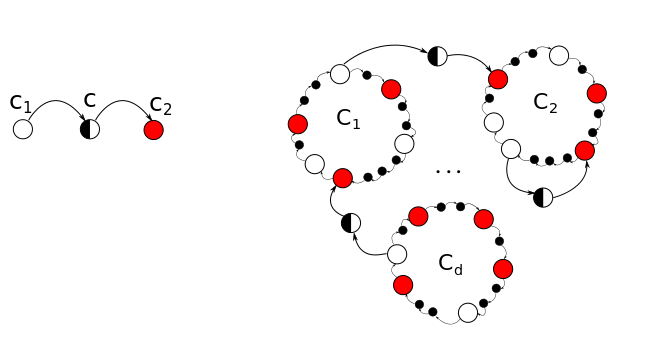
\includegraphics[scale=0.4]{GraphScheme2.png} 
\caption{Класс графов переходов (Шаг 2). Слева~--- шаблон соединения выходной и входной вершин. Справа~--- пример получаемого графа после шага 2. Полузакрашенные вершины~--- сторонние вершины, не принадлежащие ни одному кластеру $C_1$, $C_2$, $\ldots$ $C_d$}
\label{GraphSchemeTwo}
\end{figure}

\item Каждая сторонняя вершина, получаемая на шаге $2$, может быть соединена похожим образом с входной вершиной некоего кластера $C_j$: то есть посредством новой (еще не учавствовавшей в построении графа) сторонней вершины и двух новых ребер, или же посредством уже существующей сторонней (не входящей ни в один из кластеров) вершины и всего одного нового ребра (Рис.~\ref{GraphSchemeTree}).

\begin{figure}[h]
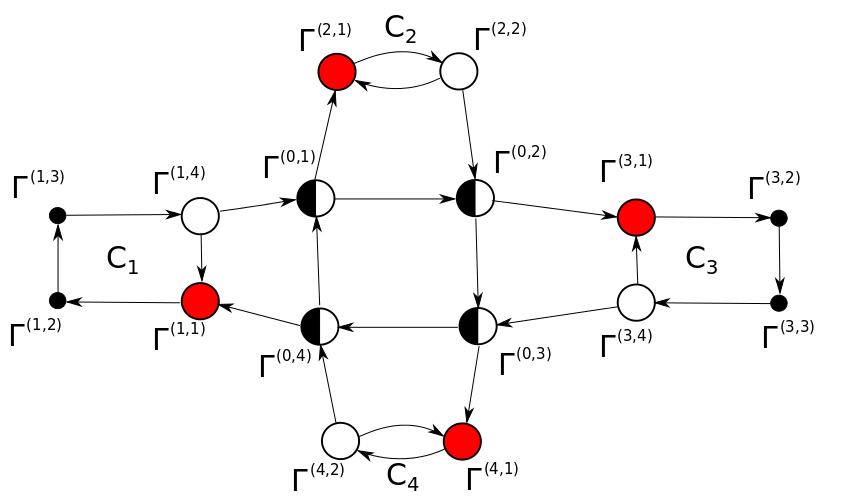
\includegraphics[scale=0.5]{GraphScheme3.png} 
\caption{Класс графов переходов (Шаг 3)}
\label{GraphSchemeTree}
\end{figure}
\end{enumerate}

Стоит отметить, что шаг $3$ может повторяться неоднократно, но конечное число раз.
 
Последнее требование, которое будет наложено заключается в следующем. Изо всех выходных вершин кластеров должны выходить ровно два ребра, ровно как во входные вершины кластеров должно входить также ровно два ребра; что касается сторонних вершин, то и из любой сторонней вершины должны выходить также по два ребра.
















\subsection{Кибернетический подход к изучению систем массового обслуживания с управлением}
Теперь перейдем к описанию основного метода, используемого в данной работе для исследования построенной модели. Не вдаваясь в данном разделе в математические детали, сформулируем основную задачу теории массового обслуживания и некоторые наиболее известные подходы к ее решению. 

Математической моделью системы обслуживания, как правило, является случайный процесс $\brrr{\xi(t) \colon t \in T}$ такой, что случайная величина $\xi(t)$ задает состояние системы в момент $t \in T$. Задача исследовтеля заключается в том, чтобы восстановить по физическому описанию системы вероятностное распределение этого процесса и изучить свойства распределения. Обозримость решения этой задачи во многом зависит от выбора описания состояния системы. В классических работах по данной тематике, например, изучались длина очереди, время ожидания начала обслуживания произвольного требования, число занятых линий. В связи с созданием и развитием А.А.~Боровковым асимптотических методов анализа в теории массового обслуживания в его работах система описывается трехмерным случайным процессом $\brrr{\eta(t), \nu(t), \zeta(t)\colon t \geqslant 0}$, в котором компоненты $\eta(t)$, $\nu(t)$ и $\zeta(t)$ соответственно определяют число поступивших, число получивших отказ и число обслуженных требований за промежуток $[0;t)$. 

Далее, кроме процесса $\brrr{\xi(t) \colon t \in T}$ рассматривают также процесс $\brrr{u(t) \colon t \in T}$, интерпретируемый как управление системой обслуживания. Управление может быть и случайным элементом, и детерменированной величиной. Ограничения на множество всех допустимых управлений имеют различную природу: математическую (например, измеримость), физическую (например, непрерывность), специфика задачи (например, в задачах о назначении приоритетов при обслуживании разнотипных требований).

Таким образом, математик -- исследователь управляемой системы массового обслуживания должен решать непростую задачу по описанию управляемого случайного процесса $\brrr{(\xi(t), u(t)) \colon t \in T}$. Упомянутые подходы обладают тем недостатком, существенно затрудняющими их применение для реальных систем, что достигаемая ими математическая общность не дает возможности принять в расчет многие физические особенности конкретных систем и построить конечномерные распределения рассматриваемого случайного процесса $\brrr{(\xi(t), u(t)) \colon t \in T}$.

В связи с вышесказанным, в данной работе будет применен другой подход, который с единых позиций рассматривает любую управляемую систему. Этот подход называется кибернетическим. Он базируется на трех постулатах. Во--первых, система массового обслуживания, как и многие другие кибернетические системы, функционирует в дискретном времени. Действительно, моменты поступления требований, моменты окончания обслуживания и другие события образуют дискретную совокупность точек на временной оси. Поэтому следует в первую очередь выбрать дискретную временную шкалу $T=\brrr{\tau_0, \tau_1, \ldots}$ и привязывать к ней все другие рассматриваемые величины и объекты. 

Во--вторых, описание состояния элементов системы в любой момент времени $t \geqslant 0$ даже для простых законов распределения входных потоков и длительностей обслуживания приводит к сложным математическим проблемам. Локальный принцип не учитывает в полной мере физическую природу процесса обслуживания и такие важные возможности и особенности действующих систем, как функции ориентации и переналадок, неоднородность требований, изменчивость с течением времени вероятностной структуры входных потоков и длительностей обслуживания, адаптивность логической структуры обслуживающего устройства, наконец, конфликтность ситуаций в управлении и обслуживании. Итак, описание поэлементного строения системы должно быть нелокальным.

В--третьих, следует выбрать уровень детализации, на котором рассматривается система. Исторически первым был метод анализа и синтеза. Сложная система мысленно расчленялась на свои составляющие и каждая часть изучалась отдельно во всей своей полноте. Затем знание обо всех частях соединялось, синтезировалось в знание обо всей совокупности, объединенной в систему. Проблемы, возникающие при таком подходе, уже обсуждались выше. Это и огромное число составляющих, и невозможность полного описания одной части без учета ее взаимодействия с другими частями. Другой подход, появившийся лишь в $\mathrm{\Rmnum{20}}$ веке, носит название <<черный ящик>>. Исследователь вовсе не интересуется устройством системы, а пытается лишь подобрать зависимость <<выхода>> системы от ее <<входа>>. Напротив, кибернетический подход отдает дань умеренности. Считается, что каждая управляемая система обладает схемой, на которой присутствуют элементы небольшого числа типов: 1) внешняя среда, 2) полюса --- точки взаимодействия системы со средой, 3) внешняя и внутренняя память, 4) устройства по переработке информации во внешней и внутренней памяти. Память состоит из ячеек с дискретным множеством состояний. Информацией является совокупность состояний всех ячеек памяти в данный момент времени. Расположение элементов на схеме описывают координаты. Благодаря им система может воздействовать на саму себя в соответствии со своими функциональными свойствами. Функция системы определяет поведение системы массового обслуживания. Она указывает то действие, которое система может совершать, переходя к следующему моменту времени. Таким образом, под состоянием $\xi(\tau)$ системы можно понимать состояния указанных элементов в момент времени $\tau \in T$, и требуется формализовать функцию системы путем совместного рассмотрения поэлементного строения системы и ее функционирования во времени. 

Более подробно и применительно к рассматриваемой задаче кибернетический подход будет описан в следующих разделах. Будет построена математическая модель управляемой системы массового обслуживания в виде счетных управляемых марковских цепей.


